\documentclass{amsart}
\usepackage{amsmath,amsfonts,amssymb,amsthm}
\usepackage{graphicx}
\usepackage{xcolor}
\usepackage{wrapfig}
\usepackage{url}
\usepackage{caption}
\usepackage{subcaption}
\usepackage[justification=centering]{caption}

\usepackage{algorithm} % Must be loaded *after* hyperref
\usepackage[noend]{algpseudocode}

\newtheorem{theorem}{Theorem}[section]
\newtheorem{lemma}[theorem]{Lemma}

\DeclareMathOperator*{\argmax}{argmax}

\newcommand{\bigzero}{\mbox{\normalfont\Large\bfseries 0}}


\title{The dynamics of factored state hidden Markov models}
\date{1 December 2020}

\begin{document}

\maketitle

\section{Introduction and Notation}\label{sec:intro}

\subsection{Classical hidden Markov models}
In what follows we denote random variables with upper case Latin letters like 
$X$, the probability distributions from which they are drawn with calligraphy 
letters like $\mathcal X$ and specific values with lower case Latin letters like $x$.  Suppose we have a sequence of observations, 
\[
X_{1:T} := X_1,...,X_T
	\]I'm 
where at each time $t$, the observation $X_t$ can be decomposed into its 
categorical and continuous components, that is 
\begin{eqnarray}\label{eqn:decomposition}
X_t = W_t\oplus V_t
\end{eqnarray}
where $W_{t}$ is drawn from the categorical space
\[ 
\mathcal W = \{1,...,D\}
\]
and $V_t$ is drawn from a $K$ dimensional Gaussian distribution, $\mathbb R^K$.
A hidden Markov model (HMM) is a latent state model that captures the Markov dynamics of a latent process underlying the observed data.  In its most basic form, the HMM models a sequence of hidden states
\[
Z_{1:T} := Z_1,...,Z_T
\]
corresponding to $X_{1:T}$, where for any time $t$, the hidden state $Z_t$ is 
drawn from the discrete\footnote{Hidden states can of course be drawn from more complicated probability 
distributions -- see, for example, Chapter 13 of Bishop's canonical text on the 
topic \cite{B06}.  For sake of brevity, this note will only 
consider the discrete hidden state space.} probability distribution
\[
\mathcal{Z} = \{h_1,...,h_N\}.
\]
The sequence of hidden states satisfy the {\em Markov property}, that is 
\[
p(Z_t\mid Z_{t-1})=p(Z_t\mid Z_{t-1},Z_{t-2},...,Z_1),
\]
and therefore form a Markov chain.  A fully parameterized HMM, denoted by 
$\Theta$, is given by a set of three probability distributions: the initial state probability, the transition probability and the 
emission probability.

For a given $\Theta$, we assume 
these three distributions have a fixed, parametric form given by 
\begin{eqnarray*}
p(Z_1=z) &=& p_1(z;\theta_1)\\
p(Z_t = z\mid Z_{t-1}=z') & = & p_z(z\mid z';\theta_z)\\
p(X_t=x\mid Z_t=z) & = &p_x(x\mid z;\theta_x),
\end{eqnarray*} 
where 
\[
\Theta = \{\theta_1,\theta_z,\theta_x\}.
\]
For $X_t$ as in equation (\ref{eqn:decomposition}) we can refine this further, 
by
\begin{eqnarray*}
p_x(x\mid z;\theta_x)& = &p_{cat}(w\mid z; \theta_{cat})\cdot p_{cont}(v\mid z; \theta_{cont})
\end{eqnarray*}
for
\begin{eqnarray*}
p(W_t=w\mid Z_t=z) & = & p_{cat}(w\mid z; \theta_{cat}),\\
p(V_t=v\mid Z_t=z) & = & p_{cont}(v\mid z; \theta_{cont}),
\end{eqnarray*}
with $\theta_x = \{\theta_{cat},\theta_{cont}\}$.
The $\theta_i$ will often be left off of the expressions above when is clear 
from context. 

The {\em initial state probability} given by $p_1$ is encoded in an $N\times 1$ 
vector describing the probabilty of inhabiting each of the $N$ hidden states at 
time $t=1$.  The $i^{th}$ term of the initial state vector is given by  
$p_1(h_i; \theta_1)$. 

The {\em transition probability}, which describes the 
likelihood of transitioning from any one state to another, is captured in an 
$N\times N$ matrix, 
\[
A=\begin{bmatrix}
a_{ij}
\end{bmatrix}_{i,j=1}^N \text{ where }a_{ij} = p_z(h_j\mid h_i;\theta_z)
\]
One relevant observation that we can make about the transition matrix, is that 
every row of $A$ necessarily sums to 1, since 
\begin{eqnarray}\label{eqn:transitionsum}
\sum_{j=1}^Np_z(h_j\mid h_i)=\sum_{j=1}^N\frac{p(h_j,h_i)}{p(h_i)}=1.
\end{eqnarray}
marginal over $h_i$.

The {\em emission probability} is the parameter that directly 
couples the observation sequence and the hidden 
state sequence and captures the probability of an observation vector given each 
of the hidden states. The categorical part of the emission probability can be 
described by a $D\times N$ matrix, 
\[
B = \left[b_{i}(d)\right]_{d,i=1}^{D,N}\text{ where }b_{i}(d) =p_{cat}(d\mid h_i; \theta_{cat}).
\]
For the continuous part of the emission probability, each hidden state, $h_i$ 
corresponds to a $K$-dimensional Gaussian distribution with a 
$K$-dimensional mean vector, $\mu_i$, 
and $K\times K$ covariance matrix, $\Sigma_i$ for each hidden state $h_i$, and 
hence 
\[
p_{cont}(v\mid 
h_i;\theta_{cont})=\frac{\exp\left(-\frac{1}{2}\left(v-\mu_i\right)^\intercal\Sigma_i^{-1}
\left(v-\mu_i\right)\right)}{\sqrt{(2\pi)^K\mid \Sigma_i\mid}}.
\]
where $^\intercal$ denotes the matrix transpose. The graphical model for a classical HMM can 
be seen in Figure \ref{fig:HMM}.  One primary goal in much of what follows, will be to learn the components of 
$\theta$.

\begin{figure}
\centering
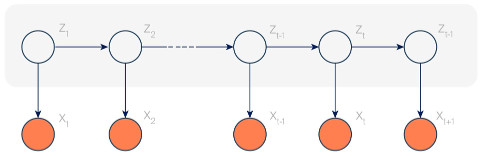
\includegraphics[scale=0.5]{figures/hmm.jpg}
\caption{The graphical model of a classical HMM}\label{fig:HMM}
\end{figure}

\subsection{Factored hidden Markov models}\label{sect:fhmm}
In an fHMM with $M$ underlying Markov systems, the hidden state, $Z_t$, at time $t$, is an $M$-dimensional vector,
\[
Z_t = (Z_{t}^{(1)},...,Z_{t}^{(M)}),
\]
drawn from the probability distribution
\[
\mathcal Z = \mathcal{Z}^{(1)}\times ...\times \mathcal{Z}^{(M)}
\]
where 
\[
\mathcal Z^{(m)} = \{h_1^{(m)},...,h_{N_M}^{(m)}\}, 
\]
for all $1\leq m\leq M$.  To simplify the exposition, we will assume throughout this note that 
\[
N = N_1 = ...= N_M
\]
although a similar narrative will hold when this restiction is removed. 

The random variable $Z_t\in \mathcal Z$ can take on one of $N^M$ possible values, 
\begin{eqnarray}\label{eqn:vec}
s_i = (s_{i}^{(1)},...,s_{i}^{(M)})\text{ where }s_i^{(m)}\in \{h_1^{(m)},...,h_{N}^{(m)}\}
\end{eqnarray}
for $1\leq i\leq N^M$.  The set of hidden 
state variables in $\mathcal Z^{(m)}$ can be more concisely 
represented by a collection of $N$ 
many $N\times 1$ matrices, each 
of which is 0 in all but one component.  In this way we can 
represent $s_i$ as the $N\times M$ matrix obtained by concatenating the 
appropriate $s_i^{(m)}$ column vectors,
\[
s_i = 
\left[
\begin{array}{c|c|c}
s_i^{(1)} &  \cdots & s_i^{(M)} 
\end{array}
\right].
\]
A comprehensive treatment of fHMMs can be found in the foundational publication 
on the topic by Gharamani and Jordan \cite{GJ95}, but we will highlight some 
key components of that paper here.  

The initial state vector, $Z_1$, can take on one of $N$ values in each of 
its $M$ components, therefore, we will define the 
initial state probability as the $M\times N$ matrix, $\pi$ where the 
entry in row $m$ and column $n$ of $\pi$ is defined as 
\begin{eqnarray*}
\pi_n^{(m)} & := & p\left(Z_1^{(m)}=h_{n}^{(m)}; \Theta\right).
\end{eqnarray*}
Under this definition, note that each row of $\pi$ necessarily sums to 
1. The transition probability will be described by a collection of $M$ many $N\times N$ matrices, 
\[
\{A^{(1)},...,A^{(M)}\},
\]
where 
\[
A^{(m)} = \begin{bmatrix}
a_{nn'}^{(m)}
\end{bmatrix}_{1\leq n,n'\leq N}
\]
with
\[
a_{nn'}^m := p(Z_t^{(m)} = 
h_{n'}^{(m)}\mid Z_{t-1}^{(m)} = h_n^{(m)}; \Theta)
\]
for $1\leq m\leq M$.  Under this definiton, for a fixed $m$, the 
rows of $A^{(m)}$ sum to 1. 

The probability of transitioning from one hidden state vector to another can 
then be constructed as a tensor product of these matrices.  More concretely, 
the probabilty of transitioning from a particular hidden state vector at time 
$t-1$ to any another hidden state vector at time $t$ can be decomposed as the product
\begin{eqnarray}\label{eqn:trans2}
p(Z_t\mid Z_{t-1}) = \prod_{m=1}^M p(Z_{t}^{(m)} \mid Z_{t-1}^{(m)}).
\end{eqnarray}
In this way each of the Markov processes evolves independently, according to 
its own dynamics. A graphical model for the fHMM can be seen in Figure 
\ref{fig:fHMM}.

\begin{figure}
\centering
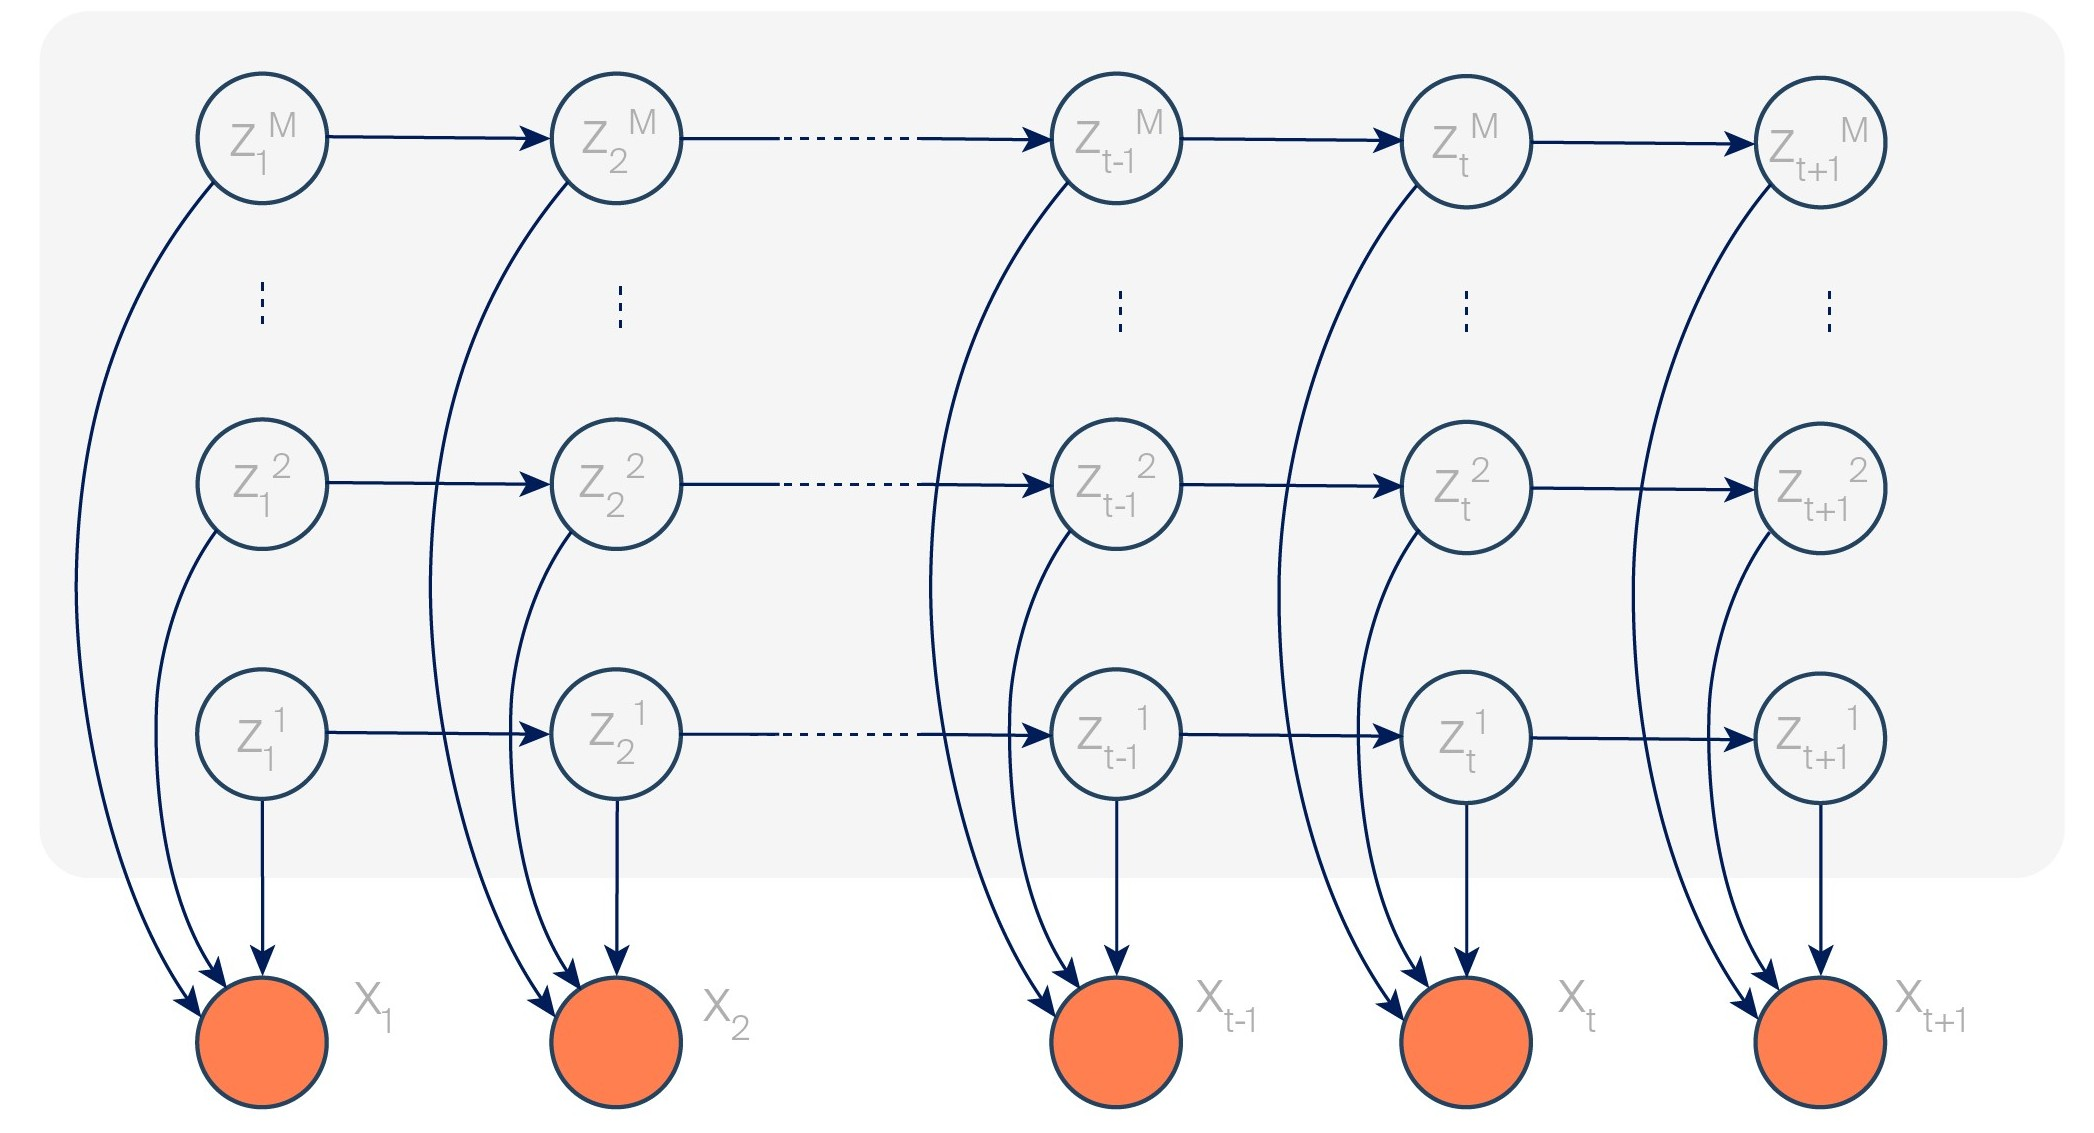
\includegraphics[scale=0.1]{figures/fhmm.jpg}
\caption{The graphical model of a factored HMM}\label{fig:fHMM}
\end{figure}

Although we want to maintain this marginal independence for the hidden states, 
$Z_{1:T}$, we would expect some dependence once we condition on the observation 
sequence, $X_{1:T}$.  In particular, the hidden values across systems 
at a fixed timestep are not independent of one another conditioned on 
the observation at the given timestep. If we consider 
the fHMM as a graphical model as in Figure (\ref{fig:fHMM}) we can couch this 
observation in the language of directed graphs and the so-called d-separation 
criterion. This conditional dependence means that, in particular, we would not expect the 
emission probability to decompose as a tensor product as in equation 
(\ref{eqn:trans2}). Intuitively, this means that the hidden state at 
one layer has the possibility to be "explained away" by the hidden 
state at another layer, an example of what is known as Berkson's 
paradox. 

Recall that an observation vector $X$ can be decomposed into its 
categorical part, $Y$, and continuous part, $V$, and 
\begin{eqnarray}
p(X_t\mid Z_t) = p(Y_t\mid Z_t)\cdot p(V_t\mid Z_t).
\end{eqnarray}
In the case of categorical observations we can 
describe the emission probability much like in the classical case, but encoding 
the information in a $D\times N^M$ matrix, $B$, where 
\[
B = \left[b_{i}(d)\right]_{d,i=1}^{D,N^M}
\]
with 
\[
b_{i}(d) := p(Y_t=d\mid Z_t = s_i;\Theta).
\]
Under this definition, the columns of $B$ must sum to 1. The situation becomes more complicated for continuous observations.  In 
particular, the mean values for each Markov system and hidden state vector are 
determined by a $K\times N$ matrix, $W^{(m)}$, where the $kn^{th}$ entry 
of $W^{(m)}$ is the contribution to the $k^{th}$ dimension by the $n^{th}$ 
hidden state vector for system $m$. For a hidden state vector, $s_i$, as in 
equation (\ref{eqn:vec}) we obtain a $K$-dimensional mean vector
\[
\mu_i = \sum_{m=1}^M W^{(m)}s_i^{(m)}
\]
which couples the hidden state vectors across the Markov systems.
Therefore, assuming a constant $K\times K$ covariance matrix, $\Sigma$, we have 
\[
p(V_t = v\mid Z_t = s_i;\Theta) = 
\frac{\exp\left(-\frac{1}{2}\left(v-\mu_i\right)^\intercal\Sigma^{-1}\left(v-\mu_i\right)\right)}{\sqrt{(2\pi)^K\mid \Sigma\mid}}.
\]
where $'$ denotes the matrix transpose.  

For the full set of model paramters, 
\[
\Theta = \{\pi,A,B,W,\Sigma\}
\]
we can now parameterize the probabilities as in the classical case, 
with
\begin{eqnarray*}
p(Z_1 = z) & = & p_1(z;\Theta)\\
p(Z_t = z\mid Z_{t-1} = z') & = & p_z(z\mid z';\Theta)\\
p(X_t = x\mid Z_t = z) & = & p_x(x\mid z;\Theta)
\end{eqnarray*}
where $\Theta$ might be omitted when it is clear from context.

\section{Learning and Inference for Factored HMMs}

\subsection{Flexible Gibbs Sampling for Factored HMMs}

In this section we will describe the components necessary to perform Gibbs 
sampling for fHMMs in a maximally flexible way following the notation set forth 
in Section \ref{sec:intro}.  

\subsubsection{Inference with Gibbs Sampling}
Suppose we already know the model parameters, 
$\Theta$, then general strategy will be to determine the most 
likely sequence of hidden states for an observation sequence, $x_{1:T}$, by iterative 
sampling.  In particular, we will begin by randomly seeding a sequence of hidden 
states, $z_{1:T}$.  We will randomly traverse the full sequence, and for each time, 
$t$, and hidden state system, $m$, we will draw a sample  
\begin{equation}\label{eqn:sample}
{z_t^{(m)'}}\sim p(Z_t^{(m)}\mid \{z_t^{(n)}:n\neq m\},z_{t-1}^{(m)}, z_{t+1}^{(m)}, x_t),
\end{equation}
eventually replacing every $z_t^{(m)}$ with ${z_t^{(m)'}}$.  With sufficient 
iterations this process will eventually converge to a reasonable approximation 
for the most likely sequence of hidden states.  In order to do this, a first 
step will be to express equation (\ref{eqn:sample}) in terms of known 
initial state, transition, and emission probabilities.  By repeated applications of Bayes' rule and marginalizing over all possible hidden 
states for time $t$ and system $m$, we obtain 
\begin{eqnarray*}
&&p(Z_t^{(m)}\mid \{z_t^{(n)}:n\neq m\},z_{t-1}^{(m)}, z_{t+1}^{(m)}, x_t)\\
& = & \frac{
p(Z_t^{(m)},\{z_t^{(n)}:n\neq m\},z_{t-1}^{(m)}, z_{t+1}^{(m)}, x_t)
}{
\sum_{z\in \mathcal Z^{(m)}}p(z,\{z_t^{(n)}:n\neq m\},z_{t-1}^{(m)}, 
z_{t+1}^{(m)}, x_t)
}\\
& = & \frac{
p_x(x_t\mid Z_t^{(m)},\{z_t^{(n)}:n\neq m\})\cdot
p_z(z_{t+1}^{(m)}\mid Z_t^{(m)})\cdot
p_z(Z_t^{(m)}\mid z_{t-1}^{(m)})
}{
\sum_{z\in \mathcal Z^{(m)}}
p_x(x_t\mid z,\{z_t^{(n)}:n\neq m\})\cdot
p_z(z_{t+1}^{(m)}\mid z)\cdot
p_z(z\mid z_{t-1}^{(m)})
}.
\end{eqnarray*}
However, we can see the random variable $Z_t^{(m)}$ is independent of the 
denominator above, and therefore is not 
relevant to the sampling. Consequently, we can sample 
\begin{equation}\label{eqn:sample2}
z_t^{(m)'}\sim p_x(x_t\mid Z_t^{(m)},\{z_t^{(n)}:n\neq m\})\cdot
p_z(z_{t+1}^{(m)}\mid Z_t^{(m)})\cdot
p_z(Z_t^{(m)}\mid z_{t-1}^{(m)}).
\end{equation}
For a fixed $x_{1:T}$ and $z_{1:T}$ we will denote this probabilty distribution 
in equation (\ref{eqn:sample2}) as a function 
\[
f_{t,m}:\mathcal Z^{(m)}\rightarrow \mathbb{R}
\]
where 
\[
f_{t,m}(z) := \begin{cases}
p_x(x_t\mid z,\{z_t^{(n)}:n\neq m\})\cdot
p_z(z_{t+1}^{(m)}\mid z)\cdot
p_1(z)& \text{ if }t=1\\
p_x(x_t\mid z,\{z_t^{(n)}:n\neq m\})\cdot
p_z(z_{t+1}^{(m)}\mid z)\cdot
p_z(z\mid z_{t-1}^{(m)})& \text{ if }1<t<T\\
p_x(x_t\mid z,\{z_t^{(n)}:n\neq m\})\cdot
p_z(z\mid z_{t-1}^{(m)})& \text{ if }t=T
\end{cases}
\]
The sampling This process is described in its totality in Algorithm \ref{alg:gibbs}.  


\begin{algorithm}
  \caption{Gibbs Sampling Algorithm\label{alg:gibbs}}
  \begin{algorithmic}[1]
    \Function{Gibbs}{model $\Theta$; data $x_{1:T}$; hidden 
    state space $\mathcal Z$; iterations 
    $R$}
    \State $\tt{z}\leftarrow \{z_1,...,z_T\}$ initialized at random where 
    $\tt{z}_t=\{z_t^{(1)},...,z_t^{(M)})\}$
    \State ${\tt r}\leftarrow 0$
	\While{${\tt r}<R$}
      \For{all ${\tt t,m}$ in $\{0,\dots, 
      T\}\times \{0,\dots, M\}$ chosen uniformly at random} 
        \State ${\tt c} \leftarrow {\tt cumsum \{f_{t,m}(z):z\in \mathcal 
        Z^{(m)}\}}$ 
        \label{eqn:alg_prob}
        \State ${\tt u}\leftarrow$ an element of $[0,1]$ chosen uniformly at 
        random
        \State ${\tt j}\leftarrow$ minimum index of ${\tt c}$ for which 
        $\tt{u}\geq c_j$
        \State ${\tt z_t^{(m)}}\leftarrow {\tt j}^{th}$ element of $\mathcal Z^{(m)}$

      \EndFor
      \State ${\tt r}\leftarrow {\tt r+1}$
      \EndWhile
      \State\Return ${\tt z}$
    \EndFunction
  \end{algorithmic}
\end{algorithm}

\subsubsection{Learning with Gibbs Sampling}\label{sec:learningGibbs}
The problem of learning with fHMMs involves finding the set of model parameters, $\Theta$, that optimize the observed data log likelihood, 
\begin{eqnarray*}
\mathcal L(\Theta;X_{1:T}) = \log p(X_{1:T}\mid \Theta).
\end{eqnarray*}
In the case of classical HMMs, this is typically done by marginalizing over the observed data likelihood
\begin{eqnarray}\label{eqn:loglikelihood}
\log p(X_{1:T}\mid \Theta) = \log\int p(X_{1:T},Z_{1:T}\mid \Theta)\,\,dZ_{1:T}
\end{eqnarray}
to find $\mathcal L$.  The integral in equation (\ref{eqn:loglikelihood}) is generally intractible, 
but fortunately there is an effective algorithm for computing the marginal likelihood that 
doesn't involve direct evaluation of the integral.  The algorithm, called 
{\em expectation-maximization} (or {\em EM}), consists of two 
fundamental steps: the expectation or {\em E}-step, and the maximization or 
{\em M}-step.  In the {\em E}-step, the expected value of the marginal probabilty is computed 
by way of an auxiliary function,
\begin{eqnarray}
Q(\Theta,\Theta') = \mathbb E_{Z_{1:T}\mid X_{1:T},\Theta'}\left[\log p(X_{1:T},Z_{1:T}\mid \Theta\right)],
\end{eqnarray}
conditioned on the observations, $X_{1:T}$ and current ``best guess" at the model parameters, $\Theta'$.  In the maximization step, we optimize $Q$ by computing 
\[
\Theta = \text{argmax}_{\Theta}Q(\Theta,\Theta').
\]
By iteratively maximizing $Q$, it's possible to find a local maximum of the likelihood function.\footnote{The fact that the this process leads to a maximal value for $\mathcal L$ is not totally obvious.  For a detailed explanation of why EM is guaranteed to converge to a locally optimal solution, the reader is directed to \cite[$\S2.2$]{HVB20}. \textcolor{red}{$\leftarrow$ It might be helpful to clean up this note and give it a permanent home.}}

In classical HMMs the $E$-step is computed across time steps by a {\em forward-backward} 
algorithm that can be carried out with time complexity $O(TN^2)$.  In the case of 
fHMMs, exact computation of the $E$-step is intractible (cf. \cite[$\S3.3$]{GJ95}).  
Although it seems the posterior probabilties could be computed across the time 
dimension without difficulty, the intractibility is a conseqence of the conditional 
dependece of the Markov systems within each time step.  As an alternative to the 
exact $E$-step, we will compute an approximate $E$-step using the probabilities 
gathered during each iteration of Gibbs sampling.  

To understand how we might approximate the $E$-step, let's consider the components of the expected value, $Q$, in the fHMM case.  Recall that for a fixed $\Theta$,  
\begin{eqnarray}\label{eqn:1}
p(X_{1:T},Z_{1:T}\mid \Theta) & = & p(Z_1)\cdot p(X_1\mid Z_1)\cdot 
\prod_{t=2}^Tp(X_t\mid Z_t)\cdot p(Z_t\mid Z_{t-1}).  
\end{eqnarray}
Therefore, 
\begin{eqnarray*}
Q(\Theta,\Theta') = \int_{Z_{1:T}}\log p(X_{1:T},Z_{1:T}\mid \Theta) 
\cdot p(Z_{1:T}\mid X_{1:T},\Theta')\,\,dZ_{1:T}
\end{eqnarray*}
can be decomposed into three components, 
\begin{eqnarray*}
Q(\Theta,\Theta') &=& \iota(\Theta,\Theta')+\beta(\Theta,\Theta')+\alpha(\Theta,\Theta'), 
\end{eqnarray*}
where $\iota$ carries the initial state information,
\begin{eqnarray}\label{eqn:iota}
\iota(\Theta,\Theta') &=& \int_{Z_{1:T}}\log p(Z_1)\cdot p(Z_{1:T}\mid 
X_{1:T},\Theta')\,\,dZ_{1:T},
\end{eqnarray}
$\alpha$ carries the transition information,
\begin{eqnarray}\label{eqn:alpha}
\alpha(\Theta,\Theta') &=& \sum_{t=2}^T\int_{Z_{1:T}}\log p(Z_t\mid 
Z_{t-1})\cdot p(Z_{1:T}\mid X_{1:T},\Theta')\,\,dZ_{1:T}.
\end{eqnarray}
and $\beta$ carries the emission information,
\begin{eqnarray}\label{eqn:beta}
\beta(\Theta,\Theta') &=& \sum_{t=1}^T\int_{Z_{1:T}}\log p(X_t\mid 
Z_t)\cdot p(Z_{1:T}\mid X_{1:T},\Theta')\,\,dZ_{1:T},
\end{eqnarray}
In what follows we will determine which quantities are necessary to exactly 
compute and maximize equations (\ref{eqn:iota}), (\ref{eqn:alpha}) and (\ref{eqn:beta}).  
Since our hidden states are drawn from a discrete probability distribution, the integrals 
in all three equations can be replaced by discrete sums.  In an effort 
to keep our notation consistent with the notation in \cite{GJ95}, for 
each $m$ we 
introduce the $N\times 1$ vector $\langle Z_t^{(m)}\rangle$ whose 
$n^{th}$ component is given by 
\begin{eqnarray}\label{eqn:bracket1}
\langle Z_t^{(m)}\rangle_n &=& p\left(Z_t^{(m)}=h_n^{(m)}\mid 
X_{1:T},\Theta'\right),
\end{eqnarray}
which is equivalent to the definiton in
\cite[Appendix B]{GJ95}. Similarly, for each $m$, we will introduce the the $N\times N$ matrix 
$\langle Z_{t-1}^{(m)}Z_t^{(m)^\intercal}\rangle$ 
where the entry in row $n$ and column $n'$ is given by 
\begin{eqnarray}\label{eqn:bracket2}
\langle Z_{t-1}^{(m)}Z_t^{(m)^\intercal}\rangle_{nn'} &=& 
p\left(Z_{t-1}^{(m)}=h_n^{(m)},Z_t^{(m)}=h_{n'}^{(m)}\mid 
X_{1:T},\Theta'\right).
\end{eqnarray}
Finally, we introduce a collection of $M\times M$ many $N\times N$ 
matrices $\langle 
Z_t^{(m)}Z_t^{(m')^\intercal} \rangle$ where the entry in row $n$ and column $n'$ is 
given by  
\begin{eqnarray}\label{eqn:bracket3}
\langle Z_t^{(m)}Z_t^{(m')^\intercal}\rangle_{nn'} &=& 
p\left(Z_t^{(m)}=h_n^{(m)},Z_t^{(m')}=h_{n'}^{(m')}\mid 
X_{1:T},\Theta'\right).
\end{eqnarray}
Since it will be helpful in what follows, we define 
\[
\delta_{i,j}=\begin{cases}
1 & \text{ if }i=j\\
0 & \text{otherwise}.
\end{cases}
\]

% ~~~~~~~~~~~~~~~~~~~~~~~~~~~~~~~~~~~~~~~~~~~~~~~~~~~~~~~~~~~~~~~~~~~~~
% ~~~~~~~~~~~~~~~~ Lemma: Initial State Update Equations ~~~~~~~~~~~~~~
% ~~~~~~~~~~~~~~~~~~~~~~~~~~~~~~~~~~~~~~~~~~~~~~~~~~~~~~~~~~~~~~~~~~~~~

\begin{lemma}\label{lemma:initial}
For a fixed set of model parameters, $\Theta'$, the function $\iota(\Theta,\Theta')$ achieves its maximum value at
\begin{eqnarray*}
\pi_n^{(m)} &=& \frac{p(Z_1^{(m)} = h_n^{(m)}\mid 
X_{1:T},\Theta')}{\sum_{n'=1}^Np(Z_1^{(m)} = h_{n'}^{(m)}\mid 
X_{1:T},\Theta')}
\end{eqnarray*}
or written equivalently in bracket notation
\begin{eqnarray}\label{eqn:updateinitial}
\pi_n^{(m)} &=&\frac{\langle Z_1^{(m)}\rangle_n}{\sum_{n'=1}^N\langle 
Z_1^{(m)}\rangle_{n'}}
\end{eqnarray}
for $1\leq m\leq M$ and $1\leq n\leq N$.
\end{lemma}

\begin{proof}
To begin, observe that equation (\ref{eqn:iota}) can be rewritten as 
\begin{eqnarray*}
\iota(\Theta,\Theta') &=& \sum_{Z_{1:T}}\log p(Z_1)\cdot p(Z_{1:T}\mid 
X_{1:T},\Theta')\\
& = & \sum_{Z_{1:T}}\log p(Z_1)\cdot p(Z_1\mid X_{1:T},\Theta')\cdot 
p(Z_{2:T}\mid Z_1,X_{1:T},\Theta')\\
& = & \sum_{Z_1} \log p(Z_1)\cdot p(Z_1\mid 
X_{1:T},\Theta')\sum_{Z_{2:T}}p(Z_{2:T}\mid Z_1,X_{1:T},\Theta')\\
& = & \sum_{Z_1} \log p(Z_1)\cdot p(Z_1\mid 
X_{1:T},\Theta')
\end{eqnarray*}
by marginalizing over $Z_{2:T}$.  Moreover, by marginalizing across the 
factored Markov systems, we can reduce this to 
\begin{eqnarray*}
\iota(\Theta,\Theta')& = & \sum_{m=1}^M\sum_{n=1}^N 
\log\pi_n^{(m)}\cdot p(Z_1^{(m)} = h_n^{(m)}\mid X_{1:T},\Theta') + ...\\
& & ...+\sum_{\stackrel{Z_1 with }{Z_1^{(m)}=h_n^{(m)}}}\log 
p(\{Z_1^{(m')}:m'\neq m\}\mid Z_1^{(m)}=h_n^{(m)})\cdot p(Z_1\mid 
X_{1:T},\Theta').
\end{eqnarray*}
Now by considering $\iota$ as a funtion with variables $\pi_n^{(m)}$ 
for $1\leq m\leq M$ and $1\leq n\leq N$, we can optimize $\iota$ using the theory of Lagrange multipliers, 
defining the auxiliary function 
\begin{eqnarray*}
L(\{\pi_n^{(m)}:1\leq m\leq M,1\leq n\leq N\}, 
\lambda_1.,,,.\lambda_m)=\iota(\Theta,\Theta')-\sum_{m=1}^M 
\lambda_m\cdot g_m(\{\pi_n^{(m)}:1\leq n\leq N\})
\end{eqnarray*}
for Lagrange multipliers $\lambda_1,...,\lambda_m$, and the system of functions 
\begin{eqnarray*}
g_m(\{\pi_n^{(m)}:1\leq n\leq N\}) = \sum_{n=1}^N \pi_n^{(m)} -1.
\end{eqnarray*}
By setting the gradient, $\nabla L$, equal to zero, we can solve for the 
values of 
$\pi_n^{(m)}$ that optimize $\iota$. For any values of $m$ and $n$, we 
have 
\begin{eqnarray}\label{eqn:partial_L_iota1}
\frac{\partial L}{\partial \pi_n^{(m)}} & = &
\frac{p(Z_1^{(m)} = h_n^{(m)}\mid X_{1:T},\Theta')}{\pi_n^{(m)}} - 
\lambda_m
\end{eqnarray}
and 
\begin{eqnarray}\label{eqn:partial_L_iota2}
\frac{\partial L}{\partial \lambda_m} & = &-1 +\sum_{n=1}^N 
\pi_n^{(m)}.
\end{eqnarray}
Combining equations (\ref{eqn:partial_L_iota1}) and 
(\ref{eqn:partial_L_iota2}) we obtain 
\begin{eqnarray*}
\pi_n^{(m)} &=& \frac{p(Z_1^{(m)} = h_n^{(m)}\mid 
X_{1:T},\Theta')}{\lambda_m}
\end{eqnarray*}
and
\begin{eqnarray*}
1 = \sum_{n=1}^N \pi_n^{(m)} = \frac{\sum_{n=1}^Np(Z_1^{(m)} = h_n^{(m)}\mid 
X_{1:T},\Theta')}{\lambda_m}
\end{eqnarray*}
and hence 
\begin{eqnarray*}
\pi_n^{(m)} &=& \frac{p(Z_1^{(m)} = h_n^{(m)}\mid 
X_{1:T},\Theta')}{\sum_{n'=1}^Np(Z_1^{(m)} = h_{n'}^{(m)}\mid 
X_{1:T},\Theta')}.
\end{eqnarray*}
which is what we wanted to show.
\end{proof}

%
% ~~~~~~~~~~~~~~~~ Lemma: Transition Update Equations ~~~~~~~~~~~~~~~~~
%

\begin{lemma}\label{lemma:transition}
For a fixed set of model parameters, $\Theta'$, the function $\alpha(\Theta,\Theta')$ 
achieves its maximum value at
\begin{eqnarray*}
a_{nn'}^{(m)} & = & 
\frac{\sum_{t=2}^Tp(Z_{t-1}^{(m)}=h_n^{(m)},Z_{t}^{(m)}=h_{n'}^{(m)}\mid 
X_{1:T},\Theta')}{\sum_{t=2}^Tp(Z_{t-1}^{(m)}=h_{n}^{(m)}\mid 
X_{1:T},\Theta')}
\end{eqnarray*}
or written equivalently in bracket notation, 
\begin{eqnarray}\label{eqn:updatetransition}
a_{nn'}^{(m)} = \frac{\sum_{t=2}^T\langle 
Z_{t-1}^{(m)}Z_t^{(m)^\intercal}\rangle_{nn'}}{\sum_{t=2}^T\langle 
Z_t^{(m)}\rangle_n},
\end{eqnarray}
for $1\leq n,n'\leq N$ and $1\leq m\leq M$.
\end{lemma}

\begin{proof}
To begin, we will observe that equation (\ref{eqn:alpha}) can be 
rewritten as 
\begin{eqnarray*}
\alpha(\Theta,\Theta') &=& \sum_{t=2}^T\sum_{Z_{1:T}}\log p(Z_t\mid 
Z_{t-1})\cdot p(Z_{1:T}\mid X_{1:T},\Theta')\\
&=& \sum_{t=2}^T\sum_{Z_{t}}\sum_{Z_{t-1}}\log p(Z_t\mid Z_{t-1})\cdot 
p(Z_t,Z_{t-1}\mid X_{1:T},\Theta')\\
& = & \sum_{t=2}^T\sum_{Z_{t}}\sum_{Z_{t-1}}\sum_{m=1}^M\log 
p(Z_t^{(m)}\mid Z_{t-1}^{(m)})\cdot p(Z_t,Z_{t-1}\mid X_{1:T},\Theta'),
\end{eqnarray*}
where the last step follows from equation (\ref{eqn:trans2}).  If we 
consider $\alpha$ as an equation in $a_{nn'}^{(m)}$ for $1\leq n,n'\leq 
N$ and $1\leq m\leq M$, we can optimize $\alpha$ using the theory of 
Lagrange multipliers by defining the auxiliary function 
\begin{eqnarray*}
&& L(\{a_{nn'}^{(m)}:1\leq n,n'\leq N,1\leq m\leq 
M\},\lambda_1,...,\lambda_M) \\
&=& \alpha(\Theta,\Theta') - \sum_{m=1}^M\lambda_m \cdot 
g_m(\{a_{nn'}^{(m)}:1\leq n,n'\leq N\})
\end{eqnarray*}
where 
\begin{eqnarray*}
g_m(\{a_{nn'}^{(m)}:1\leq n,n'\leq N\}) = -1 + \sum_{n'=1}^N a_{nn'}^{(m)},
\end{eqnarray*}
and $\lambda_1,...,\lambda_M$ are Lagrange multipliers.  By setting the 
gradient, $\nabla L$, equal to 0, we can solve for the values of 
$a_{nn'}^{(m)}$ that optimize $\alpha$.  For any choice of $n,n'$ and 
$m$, we have 
\begin{eqnarray*}
\frac{\partial L}{\partial a_{nn'}^{(m)}} &=& \frac{\partial}{\partial 
a_{nn'}^{(m)}}\left(\sum_{t=2}^T\sum_{n=1}^N\sum_{n'=1}^N\log 
a_{nn'}^{(m)}\cdot p(Z_{t-1}^{(m)}=h_n^{(m)},Z_{t}^{(m)}=h_{n'}^{(m)}\mid 
X_{1:T},\Theta')\right) - \lambda_m\\
& = & \sum_{t=2}^T\frac{p(Z_{t-1}^{(m)}=h_n^{(m)},Z_{t}^{(m)}=h_{n'}^{(m)}\mid 
X_{1:T},\Theta')}{
a_{nn'}^{(m)}} - \lambda_m
\end{eqnarray*}
and 
\begin{eqnarray*}
\frac{\partial g_m}{\partial \lambda_m} = -1+\sum_{j=1}^Na_{nn'}^{(m)}.
\end{eqnarray*}
Setting these equal to 0, we get 
\begin{eqnarray*}
a_{nn'}^{(m)} =&& 
\sum_{t=2}^T\frac{p(Z_{t-1}^{(m)}=h_n^{(m)},Z_{t}^{(m)}=h_{n'}^{(m)}\mid 
X_{1:T},\Theta')}{\lambda_m}
\end{eqnarray*}
and 
\begin{eqnarray*}
1 = \sum_{n'=1}^Na_{nn'}^{(m)} = 
\sum_{n'=1}^N\sum_{t=2}^T\frac{p(Z_{t-1}^{(m)}=h_n^{(m)},Z_{t}^{(m)}=h_{n'}^{(m)}\mid 
X_{1:T},\Theta')}{\lambda_m}
\end{eqnarray*}
and hence 
\begin{eqnarray*}
a_{nn'}^{(m)} &=& 
\frac{\sum_{t=2}^Tp(Z_{t-1}^{(m)}=h_n^{(m)},Z_{t}^{(m)}=h_{n'}^{(m)}\mid 
X_{1:T},\Theta')}{\sum_{t=2}^T\sum_{n'=1}^Np(Z_{t-1}^{(m)}=h_{n}^{(m)},Z_{t}^{(m)}=h_{n'}^{(m)}\mid 
X_{1:T},\Theta')}
\end{eqnarray*} 
but since we can marginalize over $n'$, this is just 
\begin{eqnarray*}
a_{nn'}^{(m)} & = & 
\frac{\sum_{t=2}^Tp(Z_{t-1}^{(m)}=h_n^{(m)},Z_{t}^{(m)}=h_{n'}^{(m)}\mid 
X_{1:T},\Theta')}{\sum_{t=2}^Tp(Z_{t-1}^{(m)}=h_{n}^{(m)}\mid 
X_{1:T},\Theta')},
\end{eqnarray*}
which is what we wanted to show.
\end{proof}

% ~~~~~~~~~~~~~~~~~~~~~~~~~~~~~~~~~~~~~~~~~~~~~~~~~~~~~~~~~~~~~~~~~~~~~
% ~~~~~~~~~~~~~~~~ Lemma: Emission Update Equations ~~~~~~~~~~~~~~~~~~~
% ~~~~~~~~~~~~~~~~~~~~~~~~~~~~~~~~~~~~~~~~~~~~~~~~~~~~~~~~~~~~~~~~~~~~~
\begin{lemma}\label{lemma:emission}
For a fixed set of model parameters, $\Theta'$, the function $\beta(\Theta,\Theta')$ achieves its 
maximum value at
\begin{eqnarray}\label{eqn:updatecat}
b_i(d)& = & 
\frac{\sum_{t=1}^T\delta_{Y_t,d}\cdot p(Z_t = s_i\mid 
X_{1:T},\Theta')}{\sum_{d'=1}^D\sum_{t=1}^T\delta_{Y_t,d'}\cdot p(Z_t = s_i\mid 
X_{1:T},\Theta')}
\end{eqnarray}
for $1\leq i\leq N^M$ and $1\leq d\leq D$, and the the $K\times MN$ 
matrix 
\begin{eqnarray}\label{eqn:updatemeans}
W & = & \left(\sum_{t=1}^TV_t\langle Z_t^\intercal\rangle\right)\cdot 
\left(\sum_{T=1}^T\langle 
Z_tZ_t^\intercal\rangle\right)^\dagger
\end{eqnarray}
where $W$ is the concatenation of the $W^{(m)}$ and $\dagger$ is the Moore-Penrose 
pseudo-invers, and covariance matrix 
\begin{eqnarray}\label{eqn:updatecovariance}
\Sigma & = & \frac{1}{T}\sum_{t=1}^T V_tV_t^\intercal - 
\frac{1}{T}\sum_{t=1}^T\sum_{m=1}^MW^{(m)}\langle Z_t^{(m)}\rangle 
V_t^\intercal. 
\end{eqnarray}
\end{lemma}

\begin{proof}
To begin, we will observe 
\begin{eqnarray*}
\beta(\Theta,\Theta') &=& \sum_{t=1}^T\sum_{Z_{1:T}}\log p(X_t\mid 
Z_t)\cdot p(Z_{1:T}\mid X_{1:T},\Theta')\\
&=& \sum_{t=1}^T\sum_{Z_{1:T}}\log p(X_t\mid Z_t)\cdot 
p(Z_t,Z_{1:t-1},Z_{t+1:T}\mid X_{1:T},\Theta')\\
&=& \sum_{t=1}^T\sum_{Z_t}\log p(X_t\mid Z_t)\cdot p(Z_t\mid 
X_{1:T},\Theta')\sum_{Z_{1:t-1},Z_{t+1:T}}p(Z_{1:t-1},Z_{t+1:T}\mid 
Z_t,X_{1:T},\Theta')\\
&=& \sum_{t=1}^T\sum_{Z_t}\log p(X_t\mid Z_t)\cdot p(Z_t\mid X_{1:T},\Theta')\\
&=& \sum_{t=1}^T\sum_{Z_t}\left(\log p(Y_t\mid Z_t)+\log p(V_t\mid 
Z_t)\right)\cdot p(Z_t\mid X_{1:T},\Theta')
\end{eqnarray*}
for $X_t=Y_t\oplus V_t$.  We will now proceed to optimize the categorical and continuous components separately.

For the categorical part, we have 
\begin{eqnarray*}
\beta_{cat}(\Theta,\Theta')&:=&\sum_{t=1}^T\sum_{Z_t}\log p(Y_t\mid Z_t)\cdot p(Z_t\mid X_{1:T},\Theta')\\
& = &\sum_{t=1}^T\sum_{i=1}^{N^M}\log b_{i}(Y_t)\cdot p(Z_t = s_i\mid X_{1:T},\Theta').
\end{eqnarray*}
subject to the addded constraint 
\begin{eqnarray*}
1 &=&\sum_{d=1}^Db_{i}(d).
\end{eqnarray*}
for any $i$.  If we consider $\beta_{cat}$ as a function 
in the variables $b_{i}(d)$ for $1\leq i\leq N^M$ and $1\leq d\leq D$, 
then we can define an auxiary function 
\begin{eqnarray*}
&&L(\{b_{i}(d):1\leq i\leq N^M, 1\leq d\leq 
D\},\lambda_1,...,\lambda_{N^M})\\
& = & \beta_{cat}(\Theta,\Theta') - 
\sum_{i=1}^{N^M}\lambda_i(-1+\sum_{d=1}^Db_{i}(d))
\end{eqnarray*} 
where the $\lambda_1,...,\lambda_{N^M}$ are Lagrange multipliers.  Now 
we by setting the gradient, $\nabla L$, equal to 0 we can solve for the 
values of $b_i(d)$ that optimize $\beta_{cat}$.  Taking the partial 
derivatives, we get
\begin{eqnarray*}
\frac{\partial L}{\partial b_i(d)} & = & 
\frac{\sum_{t=1}^T\delta_{Y_t,d}\cdot p(Z_t = s_i\mid 
X_{1:T},\Theta')}{b_i(d)} - \lambda_i 
\end{eqnarray*}
and 
\begin{eqnarray*}
\frac{\partial L}{\partial \lambda_i} & = & 1-\sum_{d=1}^Db_{i}(d).
\end{eqnarray*}
Setting these expressions equal to 0 we get 
\begin{eqnarray*}
b_i(d)& = & 
\frac{\sum_{t=1}^T\delta_{Y_t,d}\cdot p(Z_t = s_i\mid 
X_{1:T},\Theta')}{\lambda_i }
\end{eqnarray*}
and 
\begin{eqnarray*}
1=\sum_{d=1}^Db_{i}(d),
\end{eqnarray*}
and combining these we arrive at 
\begin{eqnarray*}
b_i(d)& = & 
\frac{\sum_{t=1}^T\delta_{Y_t,d}\cdot p(Z_t = s_i\mid 
X_{1:T},\Theta')}{\sum_{d'=1}^D\sum_{t=1}^T\delta_{Y_t,d'}\cdot p(Z_t = s_i\mid 
X_{1:T},\Theta')}
\end{eqnarray*}
which is what we wanted to show.

For the continuous part, rather than carry out the derivation from scratch, 
we will appeal to Appendix A of \cite{GJ95}.  Recall that $W^{(m)}$ is 
a $K\times N$ matrix whose $kn^{th}$ entry is the contribution to 
observation dimension $k$ for hidden state $n$ of system $m$.  Recall 
also that $V_t$ is the $K\times 1$ continuous observation vector, 
$\Sigma$ is the $K\times K$ covariance matrix, and $\langle Z_t^{(m)}\rangle$
is an $N\times 1$ vector.  Then we can simplify the continuous part of 
$\beta$ as 
\begin{eqnarray*}
\beta_{cont}(\Theta,\Theta') & = & \sum_{t=1}^T\sum_{Z_t}\log p(V_t\mid 
Z_t)\cdot p(Z_t\mid X_{1:T},\Theta')\\ 
& = & -\frac{1}{2}\sum_{t=1}^T\sum_{Z_T}(V_t-\mu_t)^\intercal\cdot 
\Sigma^{-1}\cdot (V_t-\mu_t)\cdot p(Z_t\mid X_{1:T},\Theta') - C\\
& = & -\frac{1}{2}\sum_{t=1}^TV_t^\intercal\Sigma^{-1} 
V_t-2\sum_{m=1}^MV_t^\intercal\Sigma^{-1}W^{(m)}\langle Z_t^{(m)}\rangle 
+...\\
&&\hspace{2cm}...+\sum_{m=1}^M\sum_{n=1}^Mtr\left\{W^{(m)^\intercal}\Sigma^{-1} W^{(n)}
\langle Z_t^{(n)}Z_t^{(m)^\intercal}\rangle\right\} - C
\end{eqnarray*}
where $'$ denotes the matrix transpose and $C$ is just a normalizing 
constant.  Now we can find the optimal values for the weight 
parameters, $W^{(M)}$, by taking the derivaive of $\beta_{cont}$ with 
respect to $W^{(m)}$ and setting the result equal to 0.  That is, 
\begin{eqnarray*}
\frac{\partial \beta_{cont}}{\partial W^{(m)}} & = & 
\sum_{t=1}^T\left(\sum_{n=1}^M W^{(n)}\langle 
Z_t^{(n)}Z_t^{(m)^\intercal}\rangle - V_t\langle Z_t^{(m)^\intercal}\rangle\right) = 0,
\end{eqnarray*}
which results in a $K\times MN$ matrix $W$ which is the concatenation 
of the $W^{(m)}$ and is defined by 
\begin{eqnarray*}
W & = & \left(\sum_{t=1}^TV_t\langle Z_t^\intercal\rangle\right)\cdot 
\left(\sum_{T=1}^T\langle 
Z_tZ_t^\intercal\rangle\right)^\dagger
\end{eqnarray*}
where $\dagger$ is the Moore-Penrose 
pseudo-inverse\footnote{\textcolor{red}{I'm not sure why this trace 
derivative works out...?}}. Similarly we can solve for the covariance 
matrix that optimizes $\beta_{cont}$, namely, 
\begin{eqnarray*}
\Sigma & = & \frac{1}{T}\sum_{t=1}^T V_tV_t^\intercal - 
\frac{1}{T}\sum_{t=1}^T\sum_{m=1}^MW^{(m)}\langle Z_t^{(m)}\rangle 
V_t^\intercal. 
\end{eqnarray*}

\end{proof}


% ~~~~~~~~~~~~~~~~~~~~~~~~~~~~~~~~~~~~~~~~~~~~~~~~~~~~~~~~~~~~~~~~~~~~
% ~~~~~~~~~~~~~~~~~~~~~ The Learning Algorithm ~~~~~~~~~~~~~~~~~~~~~~~
% ~~~~~~~~~~~~~~~~~~~~~~~~~~~~~~~~~~~~~~~~~~~~~~~~~~~~~~~~~~~~~~~~~~~~

\subsubsection{The Learning Algorithm}
With the update equations given explicitly in Lemmas 
\ref{lemma:initial}, \ref{lemma:transition}, and \ref{lemma:emission} we 
only need to approximate the bracket arrays 
$\langle Z_{t}^{(m)}\rangle$,
$\langle Z_{t-1}^{(m)}Z_{t}^{(m)^\intercal}\rangle$, and $\langle 
Z_{t}^{(m)}Z_{t}^{(m')^\intercal}\rangle$ to carry out an approximate 
version of {\em EM}. In what follows we will give a precise formulation 
for the algorithm, with pseudocode given in Algorithm 
\ref{alg:gibbs_learning} below.  All Python variables will be written 
in typewriter font, although some liberties will be taken with syntax. 
To begin, we set Python variables, {\tt T}, {\tt M}, {\tt N}, and {\tt 
L} corresponding to $T, M, N$ and $K$.  A hidden state at time ${\tt t}$ will be 
denoted by the ${\tt N\times M}$ array
\[
{\tt z_t} = \left[{\tt z_t^{(0)},...,z_t^{(M-1)}}\right]
\]
where each ${\tt z_t^{(m)}}$ is an ${\tt N\times 1}$ array equal to 0 
in all but one place.  The set of $M$ many $K\times K$ mean matrices 
will be stored as a $K\times M \times N\times N$ array, {\tt W}, where 
{\tt W[m]} corresponds to $W^{(m)}$.  We will initialize a ${\tt T\times M\times 
M\times N\times N}$ 
dimensional array of zeros, ${\tt \Gamma}$, where for any ${\tt t}$, 
\[
{\tt \Gamma[t][m][m']}
\]
is an ${\tt N\times N}$ array with entry ${\tt n,n'}$
corresponding to the 
${\tt n}^{th}$ hidden state of Markov system ${\tt m}$ and the ${\tt 
n'}^{th}$ hidden state of Markov system ${\tt m'}$. For each iteration 
of Gibbs sampling, we will traverse the full sequence of observations. 
For every pair in the set 
\[
{\tt P} = \{{\tt (m,m'):m\leq m'}\}
\] 
we will increment the entry of ${\tt \Gamma[t][m][m']}$ corresponding to ${\tt 
z_t^{(m)}}$ and ${\tt z_t^{(m')}}$ by one.  After a sufficient number 
of iterations, we normalize ${\tt \Gamma}$ by dividing by the total 
number of iterations, at which point we have 
\begin{eqnarray*}
{\tt \Gamma[t]} &\sim&
\left(\begin{array}{@{}c|c@{}|c@{}|c@{}}
&&&\\
  \begin{matrix}
\langle Z_{t}^{(0)}Z_{t}^{(0)^\intercal}\rangle 
  \end{matrix}
  & 
  \bigzero
  &
  & 
  \bigzero \\
  &&&\\
  \hline
  &&&\\
  \begin{matrix}
  \langle Z_{t}^{(1)}Z_{t}^{(0)^\intercal}\rangle 
  \end{matrix}
  & 
  \begin{matrix}
  \langle Z_{t}^{(1)}Z_{t}^{(1)^\intercal}\rangle 
  \end{matrix}\,\,\,
  & 
  &
  \bigzero
  \\
  &&&\\
  \hline
  &&&\\
  &
  &
  \hspace{1cm}\ddots\hspace{1cm}
  &
  \\
  &&&\\
\hline
&&&\\
\begin{matrix}
  \langle Z_{t}^{(M-1)}Z_{t}^{(0)^\intercal}\rangle 
  \end{matrix}
  &
  \begin{matrix}
  \langle Z_{t}^{(M-1)}Z_{t}^{(1)^\intercal}\rangle 
  \end{matrix}\,\,
  &
  &
\langle Z_{t}^{(M-1)}Z_{t}^{(M-1)^\intercal}\rangle \\
&&&\\
\end{array}\right),
\end{eqnarray*}
where each block above has dimenion $N\times N$, and the blocks along 
the diagonal are themselves diagonal matrices, with
\[
\Delta\langle Z_{t}^{(m)}Z_{t}^{(m)^\intercal}\rangle = \langle Z_{t}^{(m)}\rangle 
\]
for each $m$, where $\Delta$ denotes the diagonal of a matrix.  

With this, the update equation for $\pi_n^{(m)}$ given by 
equation (\ref{eqn:updateinitial}) can be closely approximated as 
\begin{eqnarray}\label{eqn:updateinitialapprox}
\pi_n^{(m)} \sim\frac{{\tt \Gamma[1][m][m][n][n]}}{{\tt sum 
\,\,\Delta\,\Gamma[1][m][m]}}.
\end{eqnarray} 
Similarly, update equation 
(\ref{eqn:updatecovariance}) from Lemma \ref{lemma:emission} can be approximated by 
\begin{eqnarray}\label{eqn:updatecovarianceapprox}
\Sigma & \sim& 
{\tt\frac{1}{T}}
{\tt sum_t}
\left[
{\tt V_t*transV_t}
\right] - 
{\tt\frac{1}{T}}
{\tt sum_{t,m} }
\left[
{\tt W[m] *\Delta\,\Gamma[t][m][m]*trans V_T}
\right],
\end{eqnarray}
where ${\tt trans}$ denotes the transpose of an array.  For the next 
part, it will be helpful to think of each ${\tt \Gamma[t]}$ as a ${\tt 
MN\times MN}$ matrix, which can be achieved by concatenating across axes 
appropriately, we will call this ``flattened" array ${\tt \Gamma\Gamma}$.  
The update equation (\ref{eqn:updatemeans}) from Lemma 
\ref{lemma:emission} can then be 
approximated by 
\begin{eqnarray}\label{eqn:updatemeansapprox}
W & \sim & \left[{\tt sum_t\,\, V_t *\Delta\,\Gamma[t]}\right] * 
\left[{\tt sum_t\,\,\Gamma\Gamma[t]@trans\,\Gamma\Gamma[t]}\right]^\dagger
\end{eqnarray}
where ${\tt @}$ denotes matrix multiplication and  
${\tt \Lambda[t]}$ and $\dagger$ denotes the Moore-Penrose 
pseudoinverse.

\begin{algorithm}
  \caption{Gibbs Approximate EM Algorithm\label{alg:gibbs_learning}}
  \begin{algorithmic}[1]
    \Function{GibbsEM}{model $\Theta$; data $x_{1:T}$; hidden 
    state space $\mathcal Z$; iterations ${\tt R}$}
    \State ${\tt \Gamma}\leftarrow$ {\tt np.zeros((T,M,N,N))}
    \State ${\tt \Xi}\leftarrow$ {\tt np.zeros((M,T-1,N,N))}
    \State ${\tt \Lambda}\leftarrow$ {\tt np.zeros((T,M**N))}
    \State $\tt{z} \leftarrow$ {\sc Gibbs}($\Theta$;$x_{1:T}$;$\mathcal 
		Z$;100) \Comment{initial burn down period}
    \State ${\tt r}\leftarrow 0$
	\While{${\tt r}<R$}
      \For{all ${\tt t}$ in {\tt range(T)} chosen uniformly at random} 
		\State increment ${\tt\Lambda[t][z_t]}$ by 1
        \For{all {\tt m} in {\tt range(M)} chosen uniformly at random}
			\If{${\tt t < T-1}$}
				\State increment ${\tt \Xi[m][t][z_t^{(m)}][z_{t+1}^{(m)}]}$ by 1
			\EndIf
			\For{all ${\tt m'}$ in ${\tt range(m+1)}$}
				\State increment ${\tt 
				\Gamma[t][m][m'][z_t^{(m)}][z_{t}^{(m')}]}$ by 1
			\EndFor
			\State Carry out steps 6-9 of Algorithm \ref{alg:gibbs}
		\EndFor
      \EndFor
      \State ${\tt r}\leftarrow {\tt r+1}$
      \EndWhile
      \State $({\tt \Gamma,\Xi,\Lambda})\leftarrow \frac{1}{R}({\tt 
      \Gamma,\Xi,\Lambda})$
      \State Update $\Theta$ according to equations 
      (\ref{eqn:updateinitialapprox})-(\ref{eqn:updatecatapprox})
      \State\Return ${\tt z},\Theta$
    \EndFunction
  \end{algorithmic}
\end{algorithm}

To approximate $\langle Z_{t-1}^{(m)}Z_{t}^{(m)^\intercal}\rangle$ we 
will begin with an ${\tt M\times (T-1) \times N\times N}$ array of zeros which we 
will call ${\tt \Xi}$.  Again, as we traverse 
the full range of observations Markov systems we will gather transition statistics.  
Specifically, at any time, ${\tt t>0}$, and Markov system, ${\tt m}$, 
the entry in row ${\tt z_{t-1}^{(m)}}$ and column ${\tt z_t^{(m)}}$ 
of ${\tt \Xi[t][m]}$ will be incremented by 1. After sufficient iterations and normalization, we have
\begin{eqnarray*}
{\tt \Xi} &\sim&
\left(\begin{array}{@{}c|c@{}|c@{}}
  \begin{matrix}
\langle Z_{0}^{(0)}Z_{0}^{(0)^\intercal}\rangle 
  \end{matrix}
  & 
  &
    \begin{matrix}
\langle Z_{0}^{(M-1)}Z_{0}^{(M-1)^\intercal}\rangle 
  \end{matrix}\\
  &&\\
  \vdots&\hspace{1cm}\hdots\hspace{1cm}&\vdots\\
  &&\\
  \begin{matrix}
\langle Z_{T-1}^{(0)}Z_{T-1}^{(0)^\intercal}\rangle 
  \end{matrix}
  & 
  &
    \begin{matrix}
\langle Z_{T-1}^{(M-1)}Z_{T-1}^{(M-1)^\intercal}\rangle 
  \end{matrix}
 \end{array}\right)
 \end{eqnarray*}
Therefore, the update equation for $a_{nn'}^{(m)}$ as given in 
equation (\ref{eqn:updatetransition}) can be approximated by 
\begin{eqnarray}\label{eqn:updatetransapprox}
a_{nn'}^{(m)}&\sim& \frac{{\tt sum_t\,\,\Xi[t][m][n][n']}}{{\tt 
sum_t\,\,\Gamma[m][t][n]}},
\end{eqnarray}
where the computation above is carried out in a suitably vectorized 
manner.

To approximate the categorical emission probabilities, we will need to 
gather one additional statistic.  Initializing ${\tt T\times N^M}$ 
array of zeros, ${\tt \Lambda}$, where each entry corresponds to one of the $N^M$ 
many possible hidden state vectors.  As we traverse the full range of 
observations, for any time ${\tt t}$ we will increment the entry of 
${\tt \Lambda}$ corresponding to ${\tt z_t}$ by 1.  After a sufficient 
number of iterations we can normalize by diving ${\tt \Lambda}$ by the 
total number of iterations, and then update equation 
(\ref{eqn:updatecat}) can be approximated by 
\begin{eqnarray}\label{eqn:updatecatapprox}
b_i(d) & \sim & \frac{{\tt sum_{Y_t = d}\,\Lambda[t][i]}}{{\tt 
sum_d\,sum_{Y_t = d}\,\Lambda[t][i]}}.
\end{eqnarray}
Of course all of the computations mentioned above can be made 
significantly more efficient through simple vectorization. 

\subsection{Structured Variational Inference}

Since computing the true log likelihood, $\mathcal L (\Theta; X_{1:T})$, 
in the case of fHMMs is typically intractible, another reasonable approach is to approximate 
the true posterior distribution, $p(X_{1:T}\mid \Theta)$, by a 
simpler distribution, a method called {\em variational inference}. For 
any distribution, $q$, it is necessarily the case that 
\begin{eqnarray*}
p(X_{1:T}) & =& 
\log\sum_{Z_{1:T}}q(Z_{1:T})\left[\frac{p(Z_{1:T},X_{1:T})}{q(Z_{1:T})}\right]\\
&\geq& 
\sum_{Z_{1:T}}q(Z_{1:T})\log \left[\frac{p(Z_{1:T},X_{1:T})}{q(Z_{1:T})}\right]
\end{eqnarray*} 
where the inequality follows from Jensen's inequality.  In this way, we 
obtain a lower bound on the posterior distribution. There are many ways 
that we could define $q$, but we employ a method of structured 
variational inference that retains some of the strucure of the full 
fHMM.  In particular, we will choose $q$ as 
\begin{eqnarray}\label{eqn:11a}
q(Z_{1:T}\mid \Phi) &=& \frac{1}{\kappa_q}\prod_{m=1}^M q(Z_1^{(m)}\mid 
\Phi)\prod_{t=2}^T q(Z_t^{(m)}\mid Z_{t-1}^{(m)}, \Phi),
\end{eqnarray}
where $\kappa_q$ is just a normalization constant and $\Phi$ is a set 
of {\em variational parameters}. Recall from previous discussion, that 
for any time $t$, the hidden state vector $Z_t^{(m)}$ is given by a 
$N\times 1$ vector which is equal to 0 in all but one component, and 
$\pi^{(m)}$ is a $1\times N$ vector. Therefore, we  
define 
\begin{eqnarray}\label{eqn:11b}
q(Z_1^{(m)}\mid \Phi) &=& 
\prod_{n=1}^N\left(\lambda_{1,n}^{(m)}\pi_n^{(m)}\right)^{Z_{1,n}^{(m)}}
\end{eqnarray}
and 
\begin{eqnarray}\label{eqn:11c}
q(Z_t^{(m)}\mid Z_{t-1}^{(m)},\Phi) = 
\prod_{n=1}^N\left(\lambda_{t,n}^{(m)}\prod_{\ell=1}^N 
\left(a_{n,\ell}^{(m)}\right)^{Z_{t-1,\ell}^{(m)}}\right)^{Z_{t,n}^{(m)}}.
\end{eqnarray}
In this case the variational paramters are given by 
\[
\Phi = \{\pi^{(m)}, a^{(m)}, \lambda_t^{(m)}\},
\]
where $\pi$ and $a$ are the initial and transition probabilities as, 
respectively, as defined in section \ref{sect:fhmm}.  To better 
understand the role of the $1\times N$ vector $\lambda_t^{(m)}$, we observe that the probability of the random 
variable $Z_{t,n}^{(m)}$ being equal to 1, under the variational
distribution $q$, would be given by,
\begin{eqnarray*}
q(Z_{1,n}^{(m)} = 1\mid \Phi) &=& \lambda_{1,n}^{(m)}\cdot \pi_n^{(m)} \\
& = &  
\lambda_{1,n}^{(m)}\cdot p(Z_{1,n}^{(m)} = 1\mid \Theta),
\end{eqnarray*}
and 
\begin{eqnarray*}
q(Z_{t,n}^{(m)}=1\mid Z_{t-1,\ell}^{(m)} =1, \Phi) &=&  
\lambda_{1,n}^{(m)}\cdot a_{n,\ell}^{(m)}\\
& = & \lambda_{1,n}^{(m)}\cdot p(Z_{t,n}^{(m)}=1\mid 
Z_{t-1,\ell}^{(m)}=1,\Theta).
\end{eqnarray*}
Recall, the goal of variational inference is to approximate 
the posterior distribution, $p$, by the variational distribution, $q$, 
comparing the equations above to equation 
(\ref{eqn:1}) (which we will reproduce here for clarity),
\begin{eqnarray*}
p(X_{1:T},Z_{1:T}\mid \Theta) & = & p(Z_1)\cdot p(X_1\mid Z_1)\cdot 
\prod_{t=2}^Tp(X_t\mid Z_t)\cdot p(Z_t\mid Z_{t-1}),
\end{eqnarray*} 
we see that the $\lambda_t^{(m)}$ are playing the role of the 
emission probabilties, $p(X_t\mid Z_t, \Theta)$, that is, 
$\lambda_t^{(m)}$ is meant to approximate the probability of a given 
emission at time $t$, given the setting of the $n^\text{th}$ component 
of the $m^\text{th}$ Markov system.  In fact, the $\lambda_t^{(m)}$ can 
be thought of as emission probabilities for a fictitious set of 
observations. 

\subsubsection{Optimizaing the variational parameters}

By performing a method of gradient descient, the variational paramters,
$\lambda_t^{(m)}$, can be optimized to bring the two 
distributions closer together.  In other words, the parameter $\lambda_t^{(m)}$ 
will be optimized to minimize the KL divergence, 
\begin{eqnarray*}
KL&:=&KL(q||p)\\
 &=& \sum_{Z_{1:T}}q(Z_{1:T})\log\left[\frac{q(Z_{1:T})}{p(Z_{1:T}\mid 
X_{1:T})}\right]\\
& = & \sum_{Z_{1:T}}q(Z_{1:T})\left[\log q(Z_{1:T}) + \log p( 
X_{1:T}) - \log p(Z_{1:T},X_{1:T})\right]\\
& = & \sum_{Z_{1:T}}q(Z_{1:T})\log q(Z_{1:T}) - 
\sum_{Z_{1:T}}q(Z_{1:T})\log p(Z_{1:T},X_{1:T}) + \log p( 
X_{1:T}) 
\end{eqnarray*} 
Let's simplify this expression term by term. For simplicity, we will define the $N\times 1$ vector $\langle 
Z_t^{(m)}\rangle$ where the $n^\text{th}$ component is given by 
\begin{eqnarray*}
\langle Z_t^{(m)}\rangle_n := q(Z_{t,n}^{(m)} = 1),
\end{eqnarray*}
the $N\times N$ array, $\langle 
Z_{t-1}^{(m)}Z_t^{(m)^\intercal}\rangle$,
defined as  
\begin{eqnarray*}
\langle Z_{t-1}^{(m)}Z_t^{(m)^\intercal}\rangle :=\langle Z_{t-1}^{(m)}\rangle\cdot\langle Z_t^{(m)^\intercal}\rangle 
\end{eqnarray*}
and the $N\times N$ array, $\langle 
Z_{t}^{(m)}Z_t^{(m')^\intercal}\rangle$,
defined as
\begin{eqnarray*}
\langle Z_{t}^{(m)}Z_t^{(m')^\intercal}\rangle := \begin{cases}
\langle Z_t^{(m)}\rangle\cdot\langle Z_t^{(m')^\intercal}\rangle & \text{ 
if }m\neq m'\\
diag\{\langle Z_t^{(m)}\rangle\} & \text{ if }m=m',
\end{cases}
\end{eqnarray*}
where $diag\{\langle Z_t^{(m)}\rangle\}$ dentoes the square matrix with 
the entries of $\langle Z_t^{(m)}\rangle$ on the diagonal.
Beginning with the first term on the right hand side of $KL$ above, substituting equations 
(\ref{eqn:11a})-(\ref{eqn:11c}) into this 
expression (and dropping $\Theta$ and $\Phi$ where it is clear from 
context), we obtain 
\begin{eqnarray*}
\sum_{Z_{1:T}}q(Z_{1:T})\log q(Z_{1:T}) 
& = & \sum_{Z_{1:T}}q(Z_{1:T})\log\left[\frac{1}{\kappa_q}\prod_{m=1}^M 
q(Z_1^{(m)}) \prod_{t=2}^T q(Z_t^{(m)}\mid Z_{t-1}^{(m)})\right]\\
& = & - \log(\kappa_q)+\sum_{Z_{1:T}}\sum_{m=1}^M\log q(Z_1^{(m)})q(Z_{1:T}) + ...\\
&& \hspace{1cm}...+\sum_{Z_{1:T}}\sum_{t=2}^T\sum_{m=1}^M \log q(Z_t^{(m)}\mid Z_{t-1}^{(m)})q(Z_{1:T})
\\
& = & - \log(\kappa_q)+
\sum_{m=1}^M\log 
\pi^{(m)}\cdot \langle Z_1^{(m)}\rangle + \sum_{t=2}^T\log A^{(m)}\cdot \langle 
Z_{t-1}^{(m)}Z_t^{(m)^\intercal}\rangle+...\\
&& \hspace{1cm}...+\sum_{t=1}^T\sum_{m=1}^M\log 
\lambda_{t}^{(m)}\cdot \langle Z_{t}^{(m)}\rangle 
\end{eqnarray*}
Expanding the second term on the right hand side of the expression 
for KL above, we obtain 
\begin{eqnarray*}
&&\sum_{Z_{1:T}}q(Z_{1:T})\log p(Z_{1:T},X_{1:T}) 
\\
& = & \sum_{Z_{1:T}}q(Z_{1:T})\left[\log p(Z_1) + \log p(X_1\mid Z_1) + 
\sum_{t=2}^T\log p(X_t\mid Z_t)+ \log p(Z_t\mid Z_{t-1})\right]
\\
& = & \sum_{m=1}^M \log 
\pi^{(m)}\cdot \langle Z_1^{(m)}\rangle 
+\sum_{t=2}^T\log A^{(m)}\cdot \langle 
Z_{t-1}^{(m)}Z_t^{(m)^\intercal}\rangle +
\sum_{Z_{1:T}}\sum_{t=1}^T\log p(X_t\mid Z_t)\cdot q(Z_t).
\end{eqnarray*}
To further simplify the last term, recall that we can split our 
observation into its $K$-dimensional continuous part, $V_t$, which is 
drawn from a Gaussian distribution, and its 
1-dimensional categorical part, $Y_t$, which can take on 1 of $D$ 
possible values. In this way, we can write $X_t$ as the direct sum, 
\[
X_t = V_t\oplus Y_t
\]
and we can split the log emission probability into its continuous and 
categorical parts as 
\[
\log p(X_T\mid Z_T) = \log p(V_t\mid Z_t) + \log p(Y_t\mid Z_t).
\]
Recalling that the continuous emission probability is given by 
\begin{eqnarray*}
p(V_t\mid Z_t) = \frac{\exp\left\{-\frac{1}{2}\left(V_t - 
\sum_{m=1}^MW^{(m)}Z_t^{(m)}\right)^\intercal\cdot \Sigma^{-1}\cdot \left(V_t - 
\sum_{m=1}^MW^{(m)}Z_t^{(m)}\right)\right\}}{\sqrt{(2\pi)^{K}\cdot 
\mid \Sigma\mid}}
\end{eqnarray*}
where $\Sigma$ is the $K\times K$ convariance matrix and $W^{(m)}$ is 
the $K\times N$ matrix indicating the contribution of each Markov 
system and state to the Gaussian mean. 
With this, the continuous log emission probability can be written as 
\begin{eqnarray*}
&&\sum_{Z_{1:T}}\sum_{t=1}^T\log p(V_t\mid Z_t)\cdot q(Z_t) \\
& = & 
-\frac{1}{2}\sum_{Z_{1:T}}\sum_{t=1}^T\left[V_t^\intercal\cdot \Sigma^{-1}\cdot 
V_t - 2\sum_{m=1}^M V_t^\intercal \cdot \Sigma^{-1}\cdot 
W^{(m)}Z_t^{(m)} \right.+...\\
&&\hspace{1cm}...+\left.\left(\sum_{m=1}^MW^{(m)}Z_t^{(m)}\right)^\intercal\cdot 
\Sigma^{-1}\cdot 
\left(\sum_{m=1}^MW^{(m)}Z_t^{(m)}\right)
\right]q(Z_t)+...\\
&&\hspace{1cm}...+ \log \left((2\pi)^K\cdot\mid 
\Sigma\mid\right)^{(-1/2)}\\
& = & 
-\frac{1}{2}\sum_{t=1}^T\left[V_t^\intercal\cdot \Sigma^{-1}\cdot 
V_t - 2\sum_{m=1}^M V_t^\intercal \cdot \Sigma^{-1}\cdot 
W^{(m)}\langle Z_t^{(m)} \rangle\right.+...\\
&&\hspace{1cm}...+\left.\sum_{m=1}^M tr\left\{W^{(m)^\intercal}\cdot \Sigma^{-1}\cdot 
W^{(m)}\cdot diag\langle Z_t^{(m)}\rangle\right\}\right.+...\\
&&\hspace{1cm}...+\left.\sum_{m=1}^M\sum_{n\neq m} 
tr\left\{W^{(m)^\intercal}\cdot \Sigma^{-1}\cdot W^{(n)}\cdot \langle 
Z_t^{(n)}\rangle\cdot \langle 
Z_t^{(m)^\intercal}\rangle\right\}\right]+...\\
&&\hspace{1cm}...+ \log \left((2\pi)^K\cdot\mid 
\Sigma\mid\right)^{(-1/2)},
\end{eqnarray*}
where $diag\{\langle Z_t^{(m)}\rangle\}$ is the $N\times N$ matrix with diagonal entries 
given by $\langle Z_t^{(m)}\rangle$.


For the categorical part, recall that $\log B$ is defined as the $D\times 
N^M$ matrix where the entry in row $d$ and column $j$ is given by 
\[
\log b_{d}(j) = \log p(Y_t = d\mid Z_t = S_j),
\]
therefore, 
\begin{eqnarray*}
&&\sum_{Z_{1:T}}\sum_{t=1}^T\log p(Y_t\mid Z_t)\cdot q(Z_t) \\
& = & 
\sum_{t=1}^T\underbrace{\sum_{Z_t}\log p(Y_t\mid Z_t^1,...,Z_t^M)\cdot 
q(Z_t)}_{\text{sums one full row of $\log B$}} \\
& = & 
\sum_{t=1}^T\sum_{m=1}^M\frac{1}{M}\underbrace{\sum_{n=1}^N
\sum_{\stackrel{Z^* \text{ s.t. } }{Z_{t,n}^{(m)} =1}}\log p(Y_t\mid Z_{t,n}^{(m)} = 
1,Z^*)}_{\text{sums one full row of $\log B$}}\cdot q(Z_{t,n}^{(m)} = 1,Z^*)\\
& = & 
\sum_{t=1}^T\sum_{m=1}^M\sum_{n=1}^N \frac{1}{M}\cdot q(Z_{t,n}^{(m)} = 1)\cdot
\sum_{\stackrel{j \text{ s.t. } }{S_{j,n}^{(m)} =1}}\log b_{Y_t}(j)\\
& = & 
\frac{1}{M}\sum_{t=1}^T\sum_{m=1}^M\overrightarrow{b^{(m)}}\cdot \langle Z_t^{(m)}\rangle.
\end{eqnarray*}
where we define $\overrightarrow{b^{(m)}}$ as the $1\times N$ vector
with the $n^\text{th}$ entry is given by
\[
\overrightarrow{b^{(m)}}_n := \sum_{\stackrel{j \text{ s.t. } }{S_{j,n}^{(m)} =1}}\log 
b_{Y_t}(j)
\]
Combining all of the above, we arrive at an expression for KL in terms 
of our $\Theta$ and $\Phi$ parameters, 
\begin{eqnarray*}
KL  & = & \sum_{t=1}^T\sum_{m=1}^M\log 
\lambda_{t}^{(m)}\cdot \langle Z_{t}^{(m)}\rangle +...\\
&  & \hspace{1cm}...-\frac{1}{2}\sum_{t=1}^T\left[V_t^\intercal\cdot \Sigma^{-1}\cdot 
V_t - 2\sum_{m=1}^M V_t^\intercal \cdot \Sigma^{-1}\cdot 
W^{(m)}\langle Z_t^{(m)} \rangle\right.+...\\
&&\hspace{2cm}...+\left.\sum_{m=1}^M tr\left\{W^{(m)^\intercal}\cdot \Sigma^{-1}\cdot 
W^{(m)}\cdot diag\langle Z_t^{(m)}\rangle\right\}\right.+...\\
&&\hspace{2cm}...+\left.\sum_{m=1}^M\sum_{n\neq m} 
tr\left\{W^{(m)^\intercal}\cdot \Sigma^{-1}\cdot W^{(n)}\cdot \langle 
Z_t^{(n)}\rangle\cdot \langle 
Z_t^{(m)^\intercal}\rangle\right\}\right]+...\\
&  & 
\hspace{1cm}...-\frac{1}{M}\sum_{t=1}^T\sum_{m=1}^M\overrightarrow{b^{(m)}}\cdot \langle Z_t^{(m)}\rangle +...\\
&  & 
\hspace{1cm}...+\sum_{t=1}^T\log p(X_t) + \log \left((2\pi)^K\cdot\mid 
\Sigma\mid\right)^{(-1/2)}- \log(\kappa_q)
\end{eqnarray*}
Now taking the derivative of the expression with respect to $\log 
\lambda_\tau^{(\ell)}$ we obtain
\begin{eqnarray*}
\frac{\partial KL}{\partial \log \lambda_\tau^{(\ell)}} &= & \langle Z_\tau^{(\ell)}\rangle +
\sum_{t=1}^T\sum_{m=1}^M\left(\log\lambda_{t}^{(m)} -V_t^\intercal \cdot \Sigma^{-1}\cdot 
W^{(m)}+\frac{1}{2}\triangle^{(m)}\right.+...\\
&&\hspace{1cm}...+\sum_{n\neq m} 
\left[W^{(m)^\intercal}\cdot \Sigma^{-1}\cdot W^{(n)}\cdot \langle 
Z_t^{(n)}\rangle\right]^\intercal-\frac{1}{M}\left.\overrightarrow{b^{(m)}}\right)\frac{\partial \langle 
Z_t^{(m)}\rangle}{\partial \log \lambda_\tau^{(\ell)}} -...\\
&&\hspace{1cm}... - \langle Z_\tau^{(\ell)}\rangle,
\end{eqnarray*}
where $\triangle^{(m)}$ denotes the diagonal entries of $W^{(m)^\intercal}\cdot \Sigma^{-1}\cdot 
W^{(m)}$ and we will use the fact that 
\[
\frac{\partial \kappa_q}{\partial \log \lambda_\tau^{(\ell)}} = 
\langle Z_\tau^{(\ell)}\rangle,
\]
which is given as equation D.4 in \cite[Appendix D]{GJ95}.  Now setting 
the coefficient in parentheses equal to 0, we can solve for 
$\lambda_t^{(m)}$, giving 
\begin{eqnarray}\label{eqn:updatelambda}
\lambda_t^{(m)^\text{ new}} & = & 
\exp\left\{\frac{1}{M}\overrightarrow{b^{(m)}}-\frac{1}{2}\triangle^{(m)} + \widetilde{V_t}^{(m)}\cdot \Sigma^{-1}\cdot 
W^{(m)}\right\} 
\end{eqnarray}
where the residual error is given by 
\begin{eqnarray*}
\widetilde{V_t}^{(m)} &=&V_t^\intercal - \sum_{n\neq m}\langle 
Z_t^{(n)^\intercal}\rangle \cdot W^{(n)^\intercal}.
\end{eqnarray*}
In this manner we can preform repeated iterations of variational 
inference until the variational distribution, $q$, converges to the 
target distribution, $p$. 

Now it only remains to compute the $\langle Z_t^{(m)}\rangle$, will be 
done using a forward-backward algorithm.  Recall that $\lambda_t^{(m)}$ 
is an observation probability assocaited to Markov system $m$ at time 
$t$, and we can think of these as emission probabilities associated to 
some fictituous set of observations, which we will denote 
$X_{1:T}^*$.  In this way,
\begin{eqnarray*}
\langle Z_{t}^{(m)}\rangle_n = q(Z_{t_n}^{(m)}\mid 
X_1^{*},...,X_T^{*})
& = & \frac{q(Z_{t,n}^{(m)},
X_1^{*},...,X_T^{*})}{\sum_{n'=1}^Nq(Z_{t,n'}^{(m)}, 
X_1^{*},...,X_T^{*})}
\end{eqnarray*}
where $q(Z_{t,n}^{(m)},X_1^{*},...,X_T^{*})$ can be decomposed as 
\begin{eqnarray*}
q(Z_{t,n}^{(m)},X_1^{*},...,X_T^{*}) &=& \alpha_t^{(m)}(n)\cdot \beta_t^{(m)}(n)
\end{eqnarray*}
with 
\begin{eqnarray*}
\alpha_t^{(m)}(n) &:=& q(Z_{t,n}^{(m)},
X_1^{*},...,X_t^{*})
\end{eqnarray*}
and 
\begin{eqnarray*}
\beta_t^{(m)}(n) &:=& q(X_{t+1}^{*},...,X_T^{*}\mid Z_{t,n}^{(m)})
\end{eqnarray*}


We will define $\alpha$ and $\beta$ recusively using the 
forward-backward algorithm (Algorithm \ref{alg:fb}).  In particular, 
for each $m$ and $n$, the forward probability, $\alpha$, will be initialized as 
\[
\alpha_0^{(m)}(n) = \lambda_{1,n}^{(m)}\cdot \pi_n^{(m)}
\]
and recursively for each $t\leq T$ as 
\[
\alpha_t^{(m)}(n) = \lambda_{t,n}^{(m)} \cdot 
    \sum_{n'=1}^Na_{n'n}^{(m)}\cdot \alpha_{t-1}^{(m)}(n)
\]
where $a_{n'n}^{(m)}$ denotes the entry in row $n$ and column $n'$ of 
the transition matrix $A^{(m)}$.  Similarly, the backward probability, 
$\beta$, will be initialized as 
\[
\beta_T^{(m)}(n) = 1
\]
and descending recursively for each value of $t\geq 0$ as 
\[
\beta_{t}^{(m)}(n) = \sum_{n'=1}^N \lambda_{t+1,n'}^{(m)}\cdot 
a_{nn'}^{(m)}\cdot \beta_{t+1}^{(m)}(n'). 
\]
In this way, we obtain 
\begin{eqnarray*}
\langle Z_{t}^{(m)}\rangle_n = \frac{\alpha_t^{(m)}(n)\cdot 
\beta_t^{(m)}(n)}{\sum_{n'=1}^N\alpha_t^{(m)}(n'
)\cdot 
\beta_t^{(m)}(n')}
\end{eqnarray*}
\begin{algorithm}
  \caption{Forward-Backward Algorithm\label{alg:fb}}
  \begin{algorithmic}[1]
    \Function{ForwardBackward}{model parameters $\pi, A$ and $ 
    \lambda_t^{(m)}$ for all $t, m$}
    \State $\tt{\alpha}\leftarrow$ empty array of 
    dimension $\tt{T\times M\times N}$.
    \State $\tt{\beta}\leftarrow$ empty array of 
    dimension $\tt{T\times M\times N}$.
    
    \For{${\tt m}$ in $\{0,...,M-1\}$}
    \For{${\tt n}$ in $\{0,...,N-1\}$}
    \State $\tt{\alpha[0,m,n]} \leftarrow \lambda_{1,n}^{(m)} \cdot
    \pi_n^{(m)}$
    
    \For{${\tt t}$ in $\{1,...,T-1\}$}
    \State{$\tt{\alpha[t,m,n]} \leftarrow \lambda_{t,n}^{(m)} \cdot 
    \sum_{n'=1}^Na_{n'n}^{(m)} \cdot \alpha[t-1,m,n']$}
	\EndFor
	\State $\tt{\beta[T,m,n]} \leftarrow 1$
	\For{${\tt t}$ in $\{T-1,...,0\}$}
	\State{$\tt{\beta[t,m,n]} \leftarrow \sum_{n'=1}^N\lambda_{t+1,n'}^{(m)} \cdot
    a_{nn'}^{(m)} \cdot \beta[t+1,m,n']$}
	\EndFor
    \EndFor
    \EndFor
    \State $\tt{\beta}\leftarrow$ empty array of 
    dimension $\tt{T\times M\times N}$.
    \For{${\tt m}$ in $\{0,...,M-1\}$}
    \For{${\tt n}$ in $\{0,...,N-1\}$}
    \For{${\tt t}$ in $\{0,...,T-1\}$}
	\State{${\tt \gamma[t,m,n]}\leftarrow \frac{\alpha[t,m,n]\cdot 
	\beta[t,m,n]}{\sum_{n'=1}^N\alpha[t,m,n']\cdot \beta[t,m,n']}$}
    \EndFor
    \EndFor
    \EndFor
    \State\Return ${\tt \gamma}$
    \EndFunction
  \end{algorithmic}
\end{algorithm}
In this way, we can iteratively update the $\lambda_t^{(m)}$.  It 
should be noted that this is only a submethod in the overall goal of 
learning model parameters. 

For the given set of model parameters we can use a modified Viterbi 
algorithm to compute the most likely sequence of hidden states.  
An fHMM comprised of $M$ Markov systems with $N$ can be treated naively 
as a classical HMM by flattening the factored states into an HMM with 
$N^M$ hidden states.  In this case, the typical Viterbi algorithm would 
have time complexity of $O(TN^{2M})$ which quickly becomes 
intractible.  On the other hand, if we were to carry out exact 
inference using the factored HMM, a Viterbi type algorithm would 
require us to consider $N^M$ possible hidde state vector configuations 
at each node giving a time complexity of $O(TMN^{M+1})$ which is even 
worse. Therefore we propose a Parallel Viterbi algorithm (Algorithm 
\ref{alg:viterbi}) which uses 
structured variational inference.  Since the factored states are 
completely decoupled, inference in this case behaves more like $M$ 
classical HMMs running in parallel, therefore this inference can be 
easily carried out with time complexity $O(TMN^2)$.

\begin{algorithm}
  \caption{Parallel Viterbi Algorithm\label{alg:viterbi}}
  \begin{algorithmic}[1]
    \Function{ParallelViterbi}{model parameters $\pi, A$ and $ 
    \lambda_t^{(m)}$ for all $t, m$}
    \State $\tt{v}\leftarrow$ empty {\tt viterbi} array of 
    dimension $\tt{T\times M\times N}$.
    \State $\tt{b}\leftarrow$ empty {\tt backpointer} array of 
    dimension $\tt{T\times M\times N}$.
    
    \For{${\tt m}$ in $\{0,...,M-1\}$}
    \For{${\tt n}$ in $\{0,...,N-1\}$}
    \State $\tt{v[0,m,n]} \leftarrow \lambda_{1,n}^{(m)} \cdot
    \pi_n^{(m)}$
    \State $\tt{b[0,m,n]} \leftarrow 0$
    
    \For{${\tt t}$ in $\{1,...,T-1\}$}
    \State{$\tt{v[t,m,n]} \leftarrow \max_{n'=1}^N\lambda_{t,n}^{(m)} \cdot 
    \sum_{n'=1}^Na_{n'n}^{(m)} \cdot v[t-1,m,n']$}
    \State{$\tt{b[t,m,n]} \leftarrow \argmax_{n'=1}^N\lambda_{t,n}^{(m)} \cdot 
    \sum_{n'=1}^Na_{n'n}^{(m)} \cdot v[t-1,m,n']$}
	\EndFor
    \EndFor
    \EndFor
    \State ${\tt bestpath} \leftarrow$ empty array of dimension 
    $M\times T$.
    \For{${\tt m}$ in $\{0,...,M-1\}$}
    \State ${\tt bestpath[m,T]\leftarrow \argmax_{n'=1}^N 
    v[T,m,n']} $
    \For{${\tt t}$ in $\{T-2,...,1=0\}$}
    \State ${\tt bestpath[m,t]} \leftarrow {\tt b[t+1,m,bestpath[m,t+1]]}$ 
    \EndFor
    \EndFor
    \State\Return ${\tt bestpath}$
    \EndFunction
  \end{algorithmic}
\end{algorithm}

\subsubsection{Learning with Structured Variational Inference}

In the case where model parameters are not already known, variational  
inference can also be used for learning.  In practice, it is known that 
the variational parameters converge to optimal values after relatively 
few iterations.  This means, that for a given set of model parameters, 
the optimization routine described in the previous sections can be 
carried out relatively quickly.  Combining this with the learning 
methods employed with Gibbs sampling, we are able to develop a learning 
algorithm using variational inferece, the details of which are given as 
pseudocode in Algorithm \ref{alg:vilearning}. The critical observation 
is that as the KL divergence gets small, the bracket values returned by 
the Algorithm \ref{alg:fb} will approximate the bracket values of the 
true posterior, equations (\ref{eqn:bracket1}) - 
(\ref{eqn:bracket3}), which are all that is necessary to carry out the steps of the approximate EM 
algorithm. 

\begin{algorithm}
  \caption{Learning with Variational Inference\label{alg:vilearning}}
  \begin{algorithmic}[1]
    \Function{LearningWithVI}{model, $\Theta$, data $X_{1:T}$, 
    number of iterations, ${\tt R}$}
    \For{${\tt r}$ in ${\tt R}$}
	\State Initialize variational parameters $\{\lambda_{t,n}^{(m)}\}$ 
	for all $t,n$ and $m$.
	\For{${\tt i}$ in range(5)}\hfill\Comment{5 should work in practice}
	\State ${\tt \gamma}\leftarrow ${\sc ForwardBackward($\Theta,\{\lambda_{t,n}^{(m)}\}$)}
	\For{${\tt t}$ in range(T)}
	\For{${\tt n}$ in range(N)}
	\For{${\tt m}$ in range(M)}
	\State $\lambda_{t,n}^{(m)\text{new}}\leftarrow $ update 
	$\lambda_{t,n}^{(m)}\leftarrow $ according 
	to (\ref{eqn:updatelambda})
	\EndFor
	\EndFor
	\EndFor
	\EndFor
	\State $\Theta^\text{new}\leftarrow$ using most recent $\gamma$, update $\Theta$ according to 
	equations (\ref{eqn:updateinitial})-(\ref{eqn:updatecovariance})
	\EndFor
    \State\Return ${\Theta^\text{new}}$
    \EndFunction
  \end{algorithmic}
\end{algorithm}


\bibliographystyle{siam}
\bibliography{references}

\end{document}

